\begin{figure}[H]
	\begin{center}
		\begin{tabular}[c]{c c c}
			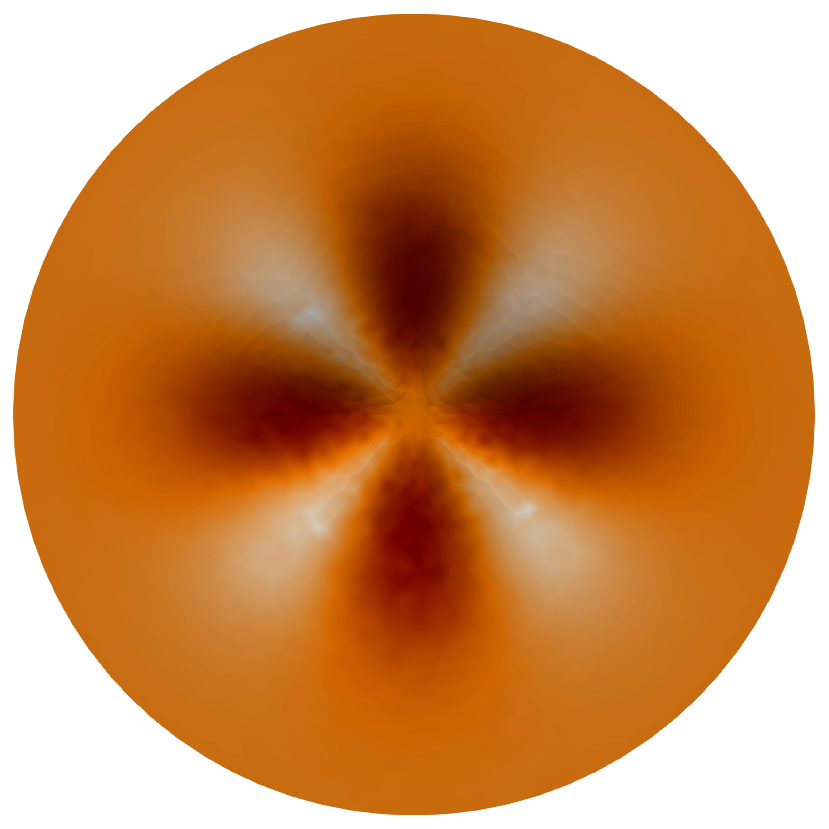
\includegraphics[scale=.15]{recoveredPressure.png} &
			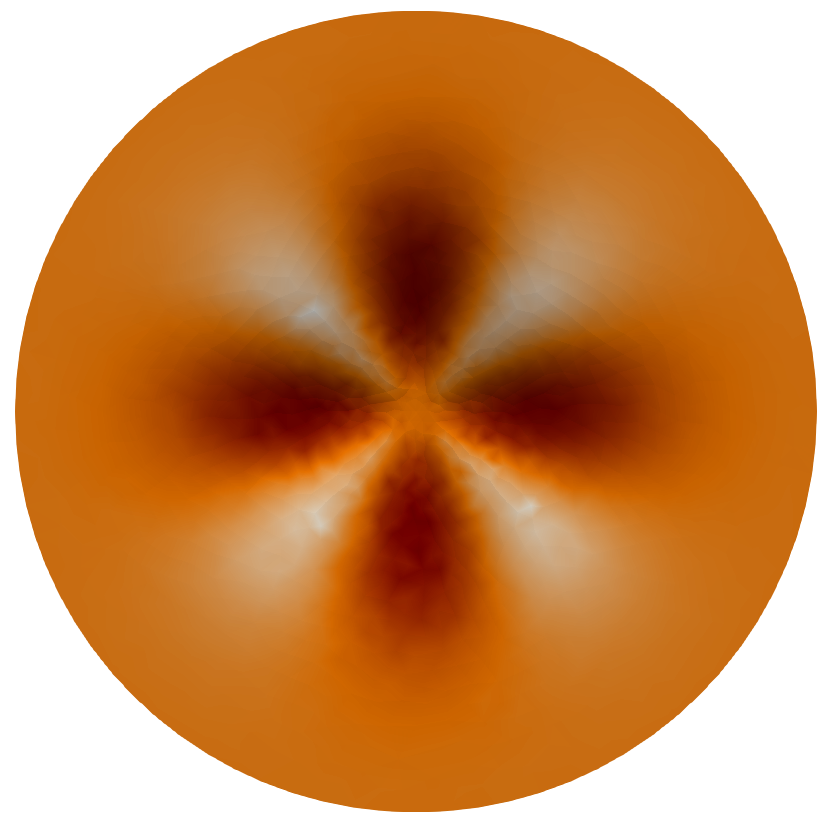
\includegraphics[scale=.15]{truePressure.png} &
			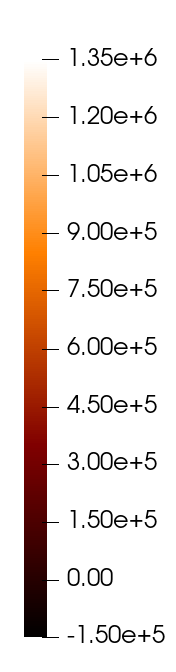
\includegraphics[scale=.18]{pressureColorBar.png} \\
			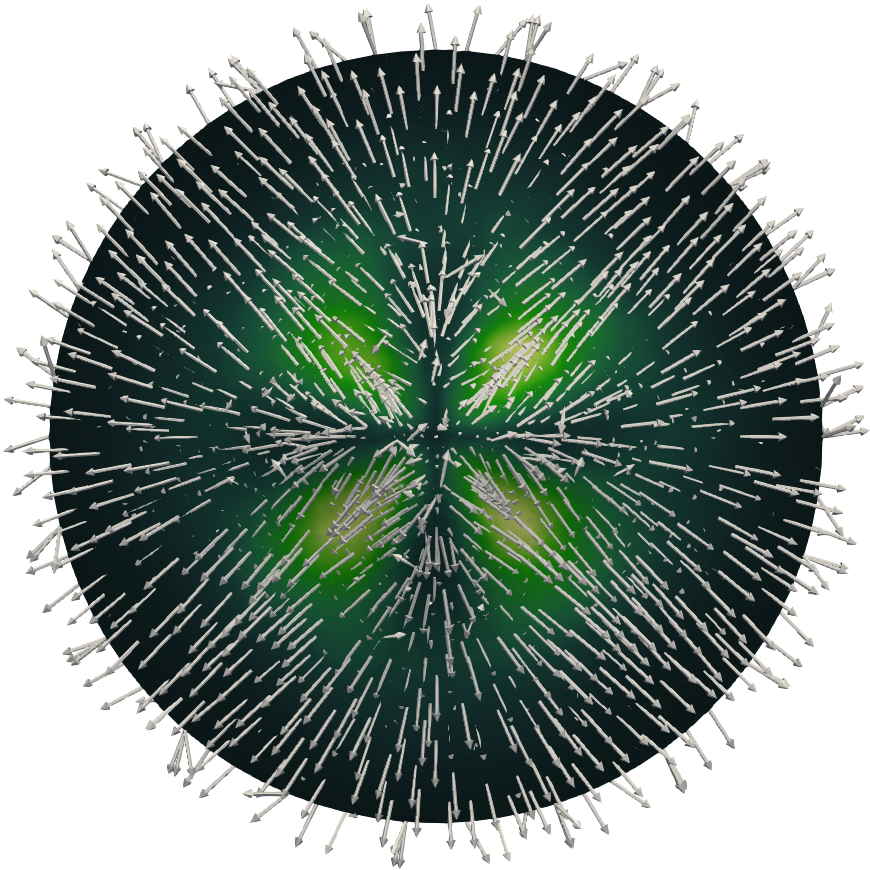
\includegraphics[scale=.15]{recoveredVelocity_glyphs.png} &
			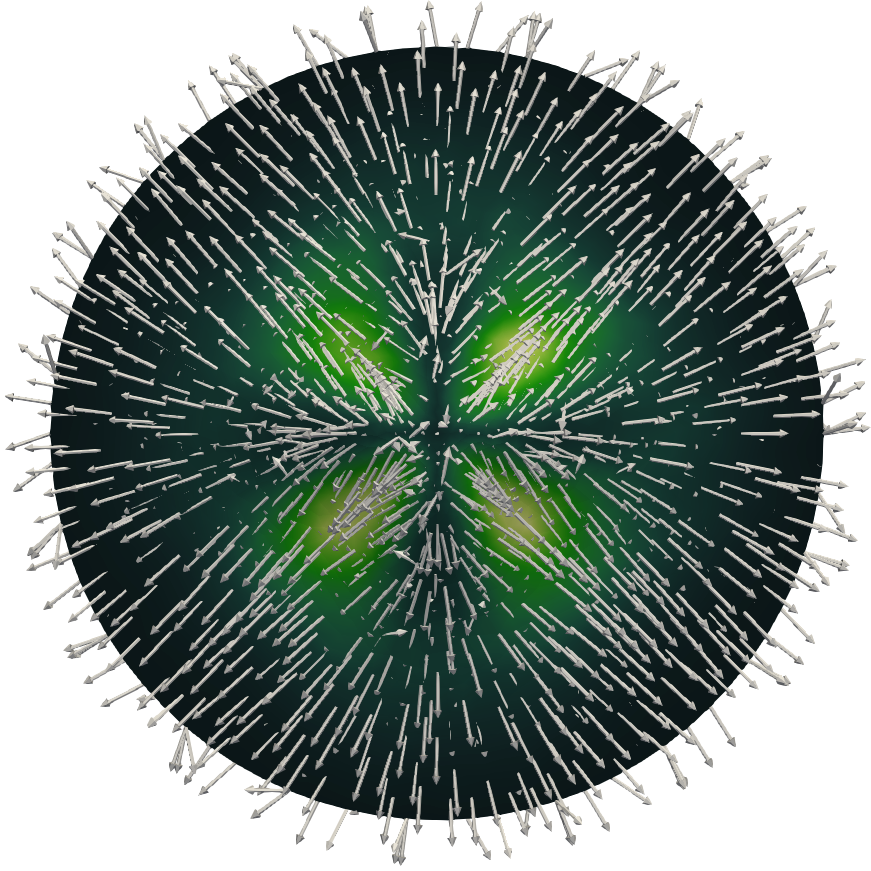
\includegraphics[scale=.15]{trueVelocity_glyphs.png} &
			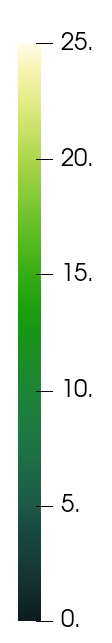
\includegraphics[scale=.18]{velocityColorBar.png} \\
			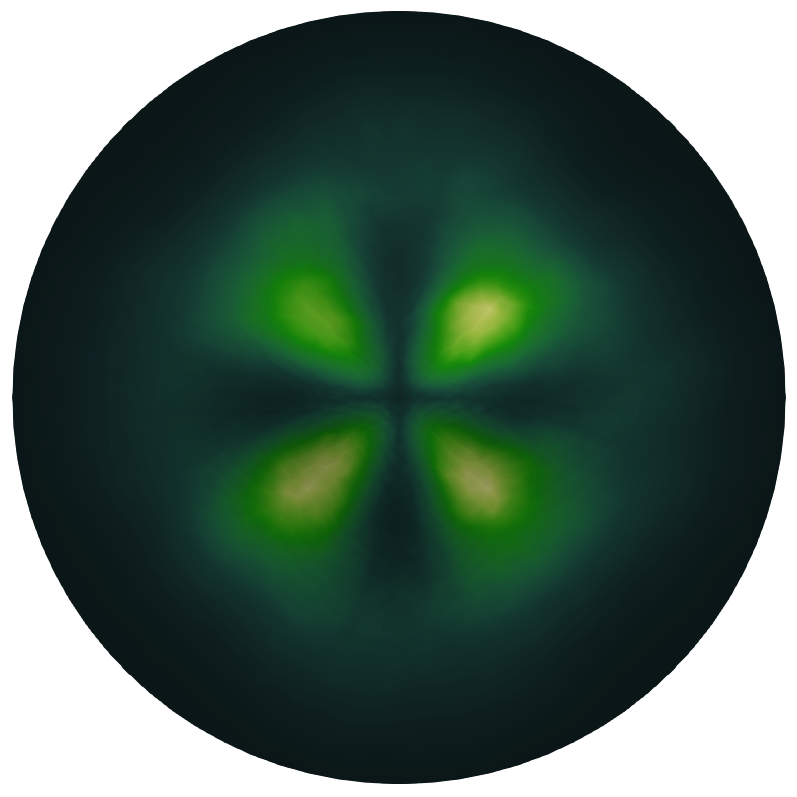
\includegraphics[scale=.15]{recoveredVelocity_noglyphs.png} &
			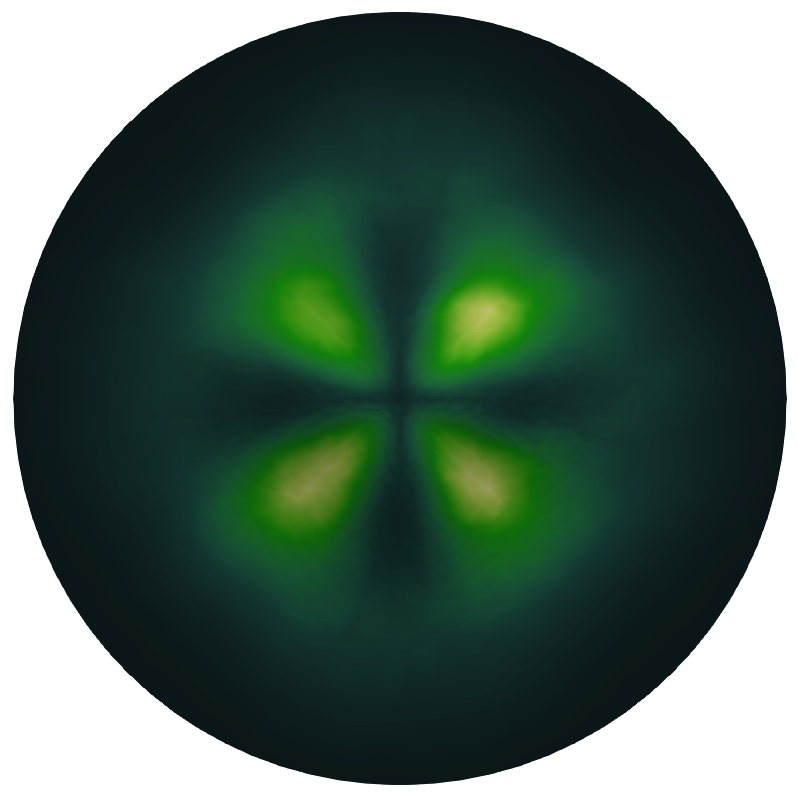
\includegraphics[scale=.15]{trueVelocity_noglyphs.png} &
			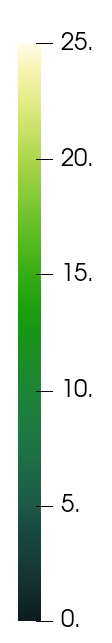
\includegraphics[scale=.18]{velocityColorBar.png}
		\end{tabular}
	\caption{Reconstructed (left column) and true (right column) pressure (top row) and velocity fields (middle and bottom rows).}
	\end{center}
\end{figure}
